\chapter{Introduction}
\label{chapter:introduction}

The research work presented in this thesis has set ambitious goal to redesign the whole well established process of data management in finite element analysis software. It also proposes efficient methods to visualize finite element meshes and the results from complex finite element analyses.

Finite Element Analysis (FEA) is the term describing the entire process of modeling the physical system using the Finite Element Method (FEM). FEA consists of model generation, meshing, attribute assignment, solution, and post-processing. With the ongoing desire to solve more complex systems with better and better precision, an analysis has to process enormous amount of data in each of its phases. Traditional unstructured file-based representation of the mesh, input parameters, and the results from the solution is the bottleneck of the entire process. It lacks the scalability and complicates the development of the tools for engineers that are either preparing the input to the FEM, or interpreting the output from the FEM.

The solution of large-scale Finite element analysis itself can be parallelized and calculated in reasonable time on high-performance computing clusters. Nevertheless, in the end the results are transfered over network and post-processed on an ordinary personal computer. Another concern is the colaboration and sharing of the model and the results between engineers and researchers. Limitations of the standard file-based approach lead to re-think the entire process of data management in FEA. The focus of the thesis is mainly on the post-processing of the results, and the way the results are stored, transfered, and visualized. However, the storage format for the results was designed with the whole picture in mind and there is proposed database-centric environment for complete FEA data management.

As an motivation example can serve the analysis of reactor vessels in nuclear power plants which is used in the process of prolongation of their service life (see Figure \ref{fig:motivation-example}). The vessels are approximately 40 years old and detailed thermo-hydro-mechanical analysis has to be performed. Usually, two-dimensional axisymmetric or fully three-dimensional models are considered and it means hundreds of thousands degrees of freedom are used. The number of time steps is between 10,000 and 15,000. The output files contain displacements, strain and stress components, temperature, relative humidity (or moisture content) and several internal parameters (e.g. creep strains, damage parameter, etc.) in all time steps. The output files with size in the order of gigabytes are generated. More details can be found in \cite{Kruis2010,Krejci2015}.

\begin{figure}[H]
\centering
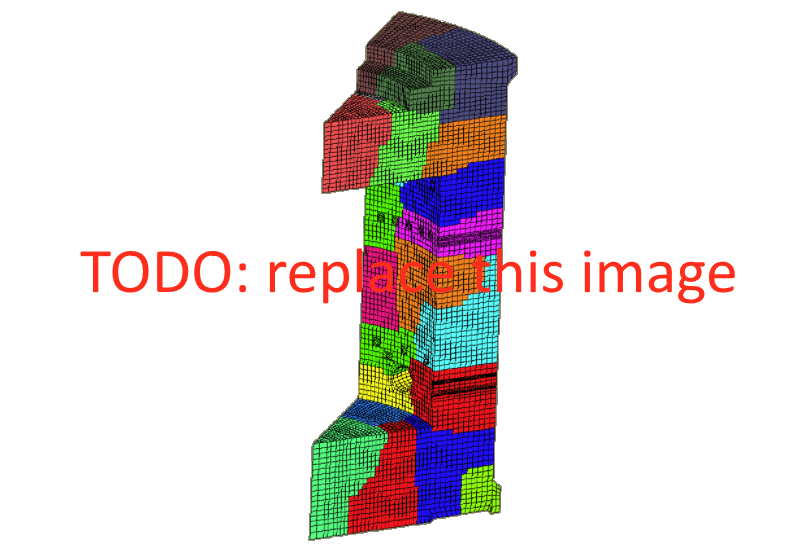
\includegraphics[width=\textwidth]{figures/chapter-introduction/motivation-example}
\decoRule
\caption[\todo{TODO:}]{\todo{TODO: Motivation example visualization}}
\label{fig:motivation-example}
\end{figure}

The thesis is structured in the following manner. Chapter \ref{chapter:related-work} gives a brief revision of related work performed in FEA data management, file formats, data compression, and post-processing of the results. Chapter \ref{chapter:data-management} deals with the alternative to file-based data management. Section \ref{sec:system-architecture} contains a proposal of relational database model that connects all parts of Finite element analysis including geometry, model attributes, and simulation results, providing query interface and remote access over the Internet. Section \ref{sec:storage-format} describes details of the new data format. Section \ref{sec:postprocessing} presents the design of the post-processor that is built on top of the data management system. Section \ref{sec:implementation-details} summarizes interesting technical details and challenges that arose during implementation of the management system and post-processor. Chapter \ref{chapter:overall-results} evaluates the implementation of the tools that are based on the new storage format and contains comparison to the traditional data formats. Chapter \ref{chapter:conclusion} concludes the thesis with final remarks, benefits and weaknesses of the chosen solution, and possible future work.

%----------------------------------------------------------------------------------------
%	SECTION Concepts
%----------------------------------------------------------------------------------------

\section{Concepts}

Here follows a summary of basic terms and concepts the thesis is based on.

\paragraph{Finite Element Method (FEM).} FEM is a numerical method for solving problems of engineering and physics. Typical areas include structural analysis, heat transfer, fluid flow, and electromagnetics. The analytical solution of these problems generally require the solution to boundary value problems for partial differential equations. The finite element method formulation of the problem results in a system of algebraic equations. The method yields approximate values of the unknowns at discrete number of points over the domain \cite{Fish2007}. To solve the problem, it subdivides a large problem domain into smaller, simpler parts that are called finite elements. This process is called the mesh generation \cite{Frey2000,Rypl1998}. The simple equations that model these finite elements are then assembled into a larger system of equations that models the entire problem. FEM then uses variational methods from the calculus of variations to approximate a solution by minimizing an associated error function. The focus of this thesis is exclusively on the data management problems in the context of FEM-based simulations, not the simulations themselves.

% TODO: do predchoziho odstavce vlozit vysvetleni gaussovych/integracnich bodu

\paragraph{Finite Element Analysis (FEA).} Various data creation and modification tasks precede and follow the actual numerical solution of the boundary value problem using FEM. This whole process is called \textbf{Finite element analysis} and consists of several distinct phases. The basic phases of a FEA depicted in Figure \ref{fig:FEA-phases} are\footnote{This is a quite simplified description of the FEA process as the results from one simulation are then sometimes used as an input for other simulations. Preliminary results of the simulation can also be post-processed continualy during the calculation phase to monitor the convergence of the iterative methods. Another case represent the iso-parametric representation of finite elements \cite{Bergheau2008}, isogeometric finite elements \cite{Hughes2005}, and NURBS-enhanced FEM \cite{Legrain2013}. These new approches are somewhat bridging the mesh generation phase as the curves describing the geometry are used also as the base functions of the finite elements.}:

\begin{enumerate}
    \item \textbf{Model creation} phase describes geometry of the domain, typically by defining boundaries of the domain using parametric surfaces like Bézier patches or Non-Uniform Rational B\'ezier-Splines (NURBS) \cite{Marsh2006} in a CAD (Computer Aided Design) tool.
    \item \textbf{Attribute definition and assignment} specifies properties of the model, i.e. material properties of volumes, initial and boundary conditions for the solution.
    \item \textbf{Mesh generation} decomposes the geometry of the model into simple shapes (triangles or quadrilaterals) or voxels like tetrahedra or bricks that fill the volume. This is often only an approximation of the orignal domain, because it is not possible for these simple shapes to fill the complex domain completely without gaps.
    \item \textbf{FEM solution} uses the equations describing the problem, model discretization, and attributes to simulate the system's behavior. Often, the process is parametric either in geometry, or in assigned attributes. Simulation then produces multiple sets of output data, each for different configuration.
    \item \textbf{Post-processing} of results is examination of the output by engineer or scientist, who is seeking the features and trends in data using the visualization tool.
\end{enumerate}

\begin{figure}[H]
    \centering
    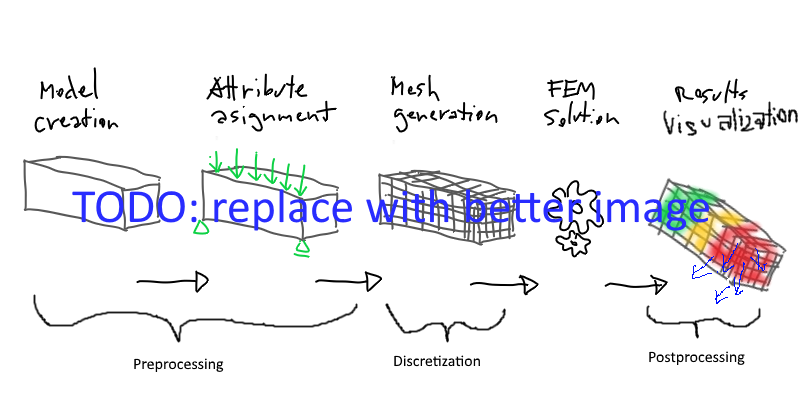
\includegraphics[width=\textwidth]{figures/chapter-introduction/FEA-phases}
    \decoRule
    \caption[\todo{TODO:}]{\todo{TODO: FEA phases}}
    \label{fig:FEA-phases}
\end{figure}

Visualization tools are used to explore and analyse the data during all the phases. However, the vast majority of discussion about FEA focuses on the solution phase only. This makes sense as the solution phase consumes the largest portion of the computer time. But the solution phase itself consumes the insignificant amount of people-time. The majority of people's time is spent in pre-processing and post-processing of complex models. This fact seems to be overlooked and is one of the motivations for research work presented in this thesis.

\paragraph{FEM results.} Results from FEM are scalar, vector, or tensor fields represented by discrete values. Some results are stored in nodes of the mesh, such as vectors of nodal displacements. Other results are stored typically in Gauss points (i.e. integration points) on finite elements. There are two similar sets of results. One is generated by a non-linear algorithms, where several incremental steps are stored and the other is generated by time integration, where results in particular time steps are stored. These results are represented as dense tabular values of basic types, usually double-precision floating-point numbers (8 bytes each). For example, a 3D material stress calculation of the domain discretized by tetrahedral elements with quadratic approximation yields 12 values for the stress and strain tensors in each Gauss points. There are 11 Gauss points in each element. If 100 time samples are taken, the size of the solution output is $100 \times 12 \times 11 \times 8 \approx 100$ kilobytes per single (!) element. The number of finite elements depends on (1) the resolution of the discretization, (2) the geometric complexity of the model, and (3) the desired accuracy of output. In practice, fine discretizations of the problem domain contain millions of elements.

Current FEA software packages store the results either sequentially in formatted \textit{ASCII or binary files} ordered by time steps, or use more sophisticated \textit{database}\footnote{The term database is used here to describe any structured storage beyond a simple file store.} systems to preserve the links between the input model and the simulation results. Either way, the size of output data is very large for non-trivial analyses, which puts pressure on storage capacity, transfer times over the network, and memory consumption of post-processing tools.

\paragraph{Data compression.} A compression method can be lossy or lossless. Lossless methods reduce information by identifying and eliminating statistical redundancy in data and are therefore able to fully reconstruct original data from its compressed form. Lossy methods, on the other hand, reduce the size by removing less important information in data and are thus producing only the approximation of original data.

\paragraph{Approximation error.} Compression methods usually yield approximated data. In the following text, the term \textit{approximation error} denotes an error resulted from compression, i.e. difference between original results of FEM analysis and their compressed form. It should not be confused with the error of the Finite Element Method itself that yields approximate solution to mathematical problems used to model physical reality. To quantify the approximation error, several error metrics were investigated. In \cite{SairaBanu2015}, there are some of them used in similar area of research. The ability to control the quality of compression was a key requirement for the implementation of the compression algorithm. There are defined several error metrics in the text (Section \ref{sec:error-estimation}) that are used to measure the approximation error.

% TODO: vysvetlit, proc pouzivam pojem Multi-mesh (Multigrid byla inspirace)

% TODO: pridat dalsi pojmy/hesla, ktera potrebuji vysvetlit. Tato kapitola by mela fungovat jako slovnicek pojmu

%----------------------------------------------------------------------------------------
%	SECTION Aims
%----------------------------------------------------------------------------------------

\section{Aims} % or Goal of the thesis

\begin{itemize}
    \item The main goal of the research work is to develop a new storage format that supports compression of results, and to outline the transition to a new post-processor that can read and visualize the compressed data in the new storage format. There is understandable resistance against invention of new data formats in the area of information technology. A new format leads to fragmentation of user base and compatibility issues. Conversion tools need to be created and maintained. There should be a strong motivation for introduction of a new format. However, there is no standard format for representation of results from FEM. Each software package uses proprietary format with syntax suitable for its internal implementation. There is also lack of support for compression methods that fit the character of FEM results. Standard file-based format does not allow for querying of specific information without the need to parse through the complete set of results. Chapter \ref{chapter:related-work} contains discussion about the existing formats in more detail and Chapter \ref{chapter:data-management} describes the proposed format.
    \item In addition, several suitable compression methods are proposed. Singular Value Decomposition (SVD) (Chapter \ref{chapter:SVD}) is the most promising method used for compression of results in this research. Other methods, that were investigated, include Wavelet transform \cite{Li2014} and approximation of discrete values by continuous polynomial functions (Chapter \ref{chapter:approximation}).
    \item Finally, the product of this research is the implementation of two post-processors. The first is the standard desktop post-processor that is based on existing software and should demonstrated the way of transition from the convential file-based formats to the proposed structured database format utilizing compression. The second post-processor is the web-based thin client intended to demonstrate the advantages of the proposed format when incorporated into a complex FEA running on a remote server.
\end{itemize}

%----------------------------------------------------------------------------------------
%	SECTION Challenges
%----------------------------------------------------------------------------------------

\section{Challenges}

Main challenge is a design of universal format that can hold the results from any FEM analysis. Results are composed of scalars, vectors, or tensors. Each field with different number of components. The results can be located on nodes or integration points. There may be a requirement to extrapolate the results from integration points to element nodes. There are different extrapolation strategies. Mesh can be different for each time step (e.g. in case of simulating the construction stages). Mesh can contain 1D, 2D, or 3D elements. Each of different type and approximation. Results from 3D simulations can be visualized on the surface of the mesh, in form of cross-sections or iso-areas, or as a vector field. The storage format should support efficient generation of all these views of results.

Finite element solution and post-processing of results can be sometimes done on different computers. Complex FEA solution phase runs on a supercomputer or a performant cluster of workstations, but the results are post-processed on common personal computer that has significantly less memory available. Typical personal computer has 8 to 16 GB of RAM available while the size of results can be in order of tens to hunderds of gigabytes. Also, the data to post-process have to be first transfered over the corporate network or the Internet. These conditions indicate the need for partitioning of data into smaller chunks and/or compression of data.

The goal of compression methods is the significant reduction in size while preserving the quality (keeping the approximation error low). Unlike with image compression methods where the main aspect is the human perception of the reconstructed image the compression of FEM results should be able to guarantee the matematical acuracy of the approximations and the user should be able to specify a desired value of the approximation error. Another concern is the computation complexity of the compression algorithm. The compression will be performed only once after the solution phase is complete. The computational time should be order of magnitude lower compared to the solution phase. Decompression (reconstruction of the original data) should be very fast as it is supposed to be performed every time the data are post-processed on the end device, which can be ordinary PC or even mobile device. The ability to create animations should also be taken into account.

Other kind of challenge is to provide the data management system that will connect all the FEA phases, i.e. to provide links between the geometric model, the mesh entities, and the output values. A project typically encompasses multiple simulations, each with different input or solver parameters. Multiple users are usually involved in the project and the system should help them to cooperate during the preparation of the input and allow to share the output of the analysis. All these aspects influence the design of the data management system.

% TODO: Pridat dalsi vyzvy a namety. Napr.:
% Slo by propojit vypocet a zpracovani vysledku? Zminit multigrid.
% Co takhle nejak zohledit chybu aproximace FEMu, zohlednit ji pri kompresi a prezentovat ji uzivateli?
